\section{Development of Algorithm to Calculate Thermal Expansion Tensors}
Calculation of a thermal expansion tensor from refined patterns collected from X-ray diffraction experiments is a complex process that will be outlined in the following sections.  The process follows the generalized steps below:
\begin{enumerate}
 \item Convert $2\theta$ values to $d$-spacing using Bragg's Law
 \item Calculate $\alpha_{hkl}$ for each $hkl$ plane listed in data
 \item Determine the thermal expansion tensor, $\alpha_{ij}$, at a single temperature using $\alpha_{hkl}$ from the previous step
 \item Determine the thermal expansion tensor for all requisite temperatures
\end{enumerate}

Bragg's law gives the angles for X-ray scattering from a crystalline lattice.  Rearranged for the purpose of this thesis, Eqn. \ref{eq:Bragg_Law} shows how $d$-spacing can be obtained from listed $2\theta$ values if wavelength, $\lambda$ is known.

\begin{equation}
 d_{hkl} = \frac{n\lambda}{2\sin\theta}
 \label{eq:Bragg_Law}
\end{equation}

\subsection{Calculation of $\alpha_{hkl}$ for $hkl$ Planes}
The concept of thermal expansion has been shown by Eqn. \ref{eq:CTE}.  It has also been mentioned that for low-symmetry crystals, multiple independent measurements of thermal expansion in many directions must be taken to determine a complete thermal expansion tensor.  When directionality is taken into account in a crystalline unit cell, thermal expansion can be modified to represent the distance between $hkl$ planes.  This representation, shown in Eqn. \ref{eq:CTE_Directional} relates the thermal expansion in a $hkl$ plane to the strain measured in the plane.  

\begin{equation}
 \alpha_{hkl} = \frac{dd_{hkl}}{d_{hkl}} \frac{1}{dT}
 \label{eq:CTE_Directional}
\end{equation}

As an example of this, Figure \ref{fig:Latparam_Trend} shows the change in thermal expansion with increasing temperature in the `$a$' lattice parameter of orthorhombic mullite ($\text{Al}_6 \text{Si}_2 \text{O}_{13}$).  A detailed analysis of this system will be provided in Chapter 4.  The visible trend in the data shows promise for the application of a mathematical model.  A search through literature revealed that H. K\"{u}ppers assigned a varying-order polynomial to a similar trend and was able to determine a thermal expansion coefficient for a high-symmetry crystal.  Eqn. \ref{eq:CTE_Polynomial} shows this relationship.  K\"{u}ppers' model is useful for high-symmetry crystals, but for low-symmetry crystals more information about off-axis expansion must be determined.

\begin{figure}[htbp]
 \begin{center}
 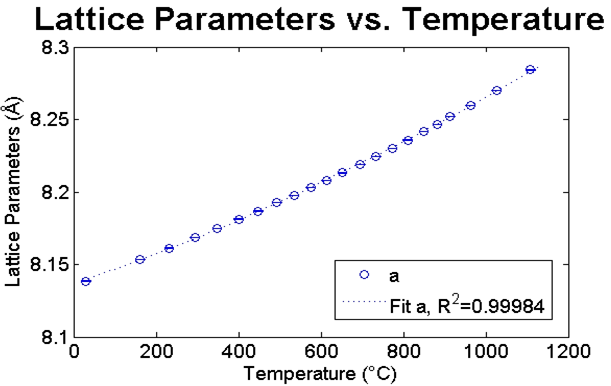
\includegraphics[width=4in,bb=0 0 358 226,keepaspectratio=true]{./Figures/Mullite_Latparams.png}
 % Mullite_Latparams.png: 611x386 pixel, 123dpi, 12.62x7.97 cm, bb=0 0 358 226
 \end{center}
 \caption{Plot of the $a$ Lattice Parameter and its Change with Increasing Temperature in Orthorhombic Mullite ($\text{Al}_6 \text{Si}_2 \text{O}_{13}$)}
 \label{fig:Latparam_Trend}
\end{figure}

\begin{equation}
 \alpha_{hkl} = \frac{dd_{hkl}}{d_{hkl}} \frac{1}{dT} = A_{n,0} + A_{n,1}T + A_{n,2}T^2
 \label{eq:CTE_Polynomial}
\end{equation}

Since data for this thesis were taken using X-ray diffraction, many more planes of expansion can be modeled with Eqn. \ref{eq:CTE_Polynomial} if the ``A'' coefficients can be determined for each $hkl$ plane.  The middle and right portions of Eqn. \ref{eq:CTE_Polynomial} show that a differential equation has been formed.  Rearranging the equation and integrating over a range of temperature yields the following relationship:

\begin{equation}
 \int_{d_{hkl,T_0}}^{d_{hkl,T}} \frac{dd_{hkl}}{d_{hkl}} = \int_{T_0}^T \left[ A_{n,0} + A_{n,1}T + A_{n,2}T^2\right]dT
 \label{eq:CTE_Integral}
\end{equation}

The solution to Eqn. \ref{eq:CTE_Integral} is shown in Eqn. \ref{eq:CTE_Solution}.  Using linear regression techniques, a value for the ``A'' coefficients can be determined.  The non-log forms of the ``A'' coefficients can then be substituted back into Eqn. \ref{eq:CTE_Polynomial} to yield a thermal expansion coefficient in a specific $hkl$ plane as a function of temperature.

\begin{equation}
 \ln d_{hkl,T} = \ln d_{hkl,T_0} + A_{n,0}\left(T-T_0\right) + \frac{1}{2} A_{n,1} \left(T-T_0\right)^2 + \frac{1}{3} A_{n,2}\left(T-T_0\right)^3
 \label{eq:CTE_Solution}
\end{equation}

\subsection{Determination of CTE Tensor from $\alpha_{hkl}$ at Temperature}

The value $\alpha_{hkl}$ is the magnitude of thermal expansion in the corresponding $hkl$ plane.  Since it is known that thermal expansion can be represented as a second-rank tensor, it is reasonable to show a relation between this magnitude of thermal expansion and the thermal expansion tensor itself.  Eqn. \ref{eq:CTE_Tensor_Calc} shows the relationship of the CTE tensor to a set of $X$, $Y$, and $Z$ coordinates in the Cartesian coordinate system.  A system of these equations can be used to solve for $\alpha_{ij}$ if $X$, $Y$, $Z$, and $\alpha_{hkl}$ are known.  $\alpha_{hkl}$ has been determined from the previous discussion based on Eqns. \ref{eq:CTE_Directional}, \ref{eq:CTE_Integral}, and \ref{eq:CTE_Solution}.

\begin{equation}
 \alpha_{hkl} = \alpha_{11} X^2 + \alpha_{22} Y^2 + \alpha_{33} Z^2 + 2\alpha_{12} XY + 2\alpha_{23} YZ + 2\alpha_{13} XZ
 \label{eq:CTE_Tensor_Calc}
\end{equation}

The $X$, $Y$, and $Z$ variables in Eqn. \ref{eq:CTE_Tensor_Calc} are in relation to a vector in Cartesian space.  Since $hkl$ planes exist in crystallographic space, a method for converting reliably between coordinate systems is necessary both to convert the planar normal of a $hkl$ plane to Cartesian coordinates and to facilitate the graphical representation of data using computer graphing utilities based in Cartesian space.

In order to solve for the $\alpha_{ij}$ coefficients in Eqn. \ref{eq:CTE_Tensor_Calc}, a system of equations equal to the number of unknown coefficients must be created.  For example, a minimum of six $hkl$ planes with corresponding $d$-spacing measurements is required to determine the $\alpha_{ij}$ coefficients in a triclinic system.  Table \ref{tbl:symmetries} can be referenced for the number of measurements based on higher symmetries.  Each $hkl$ has a planar normal that can be converted to a vector in Cartesian coordinates using Eqn. \ref{eq:ConMat}.  These Cartesian coordinates can then be used as the $X$, $Y$, and $Z$ values in Eqn. \ref{eq:CTE_Tensor_Calc}. 

\begin{equation}
 \left(
 \begin{array}{c}
 X \\
 Y \\
 Z \\
 \end{array}
 \right) =
 \left[
 \begin{array}{ccc}
  A_{1,1} & A_{1,2} & 0 \\
  0       & A_{2,2} & 0 \\
  A_{3,1} & A_{3,2} & A_{3,3}\\
 \end{array}
 \right]
 \left(
 \begin{array}{c}
  h \\
  k \\
  l \\
 \end{array}
 \right)
 \label{eq:ConMat}
\end{equation}

where,

\begin{eqnarray}
 A_{1,1} &=& a \sin \beta \nonumber \\
 A_{1,2} &=& b \left(\cos\gamma - \frac{\cos\beta\cos\alpha}{\sin\beta}\right) \nonumber \\
 A_{2,2} &=& b \left(\sin^2\alpha - \frac{A_{1,2}^2}{b^2}\right)^\frac{1}{2} \nonumber \\
 A_{3,1} &=& a \cos\beta \nonumber \\
 A_{3,2} &=& b \cos\alpha \nonumber \\
 A_{3,3} &=& c \nonumber \\
 \label{eq:ConMatEqs}
\end{eqnarray}

Eqn. \ref{eq:ConMat} is based on the resolution of the crystallographic axis system into $X$, $Y$, and $Z$ components through trigonometry.  Figure \ref{fig:Axis_Overlay} shows how this concept can be visualized.  The crystallographic coordinate system, when overlaid upon the Cartesian coordinate system shows that each axis can be resolved into components that contribute to distance along a Cartesian axis.  These sine and cosine components are the $A_{i,j}$ variables in Eqn. \ref{eq:ConMat}.  Their form follow Eqns. \ref{eq:ConMatEqs}.  

Orientation of the system relies on IEEE standards for ensuring that the $c$-axis of the crystallographic coordinate system is aligned with the $Z$-axis of the Cartesian coordinate system.  If the $\alpha$ angle in the system is $90^\circ$, the $b$-axis should align with the $Y$-axis of the Cartesian system, however the $X$-axis will lie in the $a$-$c$ plane of the crystallographic coordinate sytem.  In high symmetries where $\alpha=\beta=\gamma=90^\circ$, $X$ and $a$ are coincident as well.

\begin{figure}[htpd]
\begin{center}
 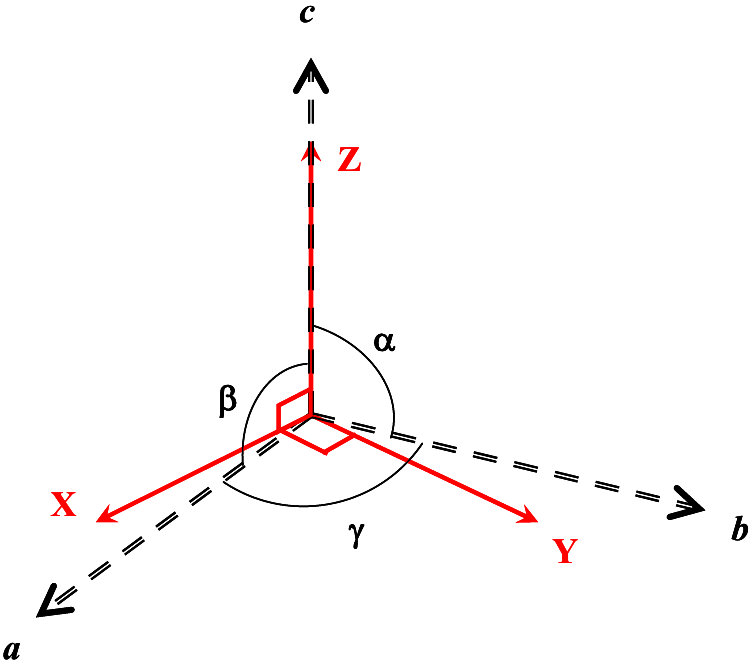
\includegraphics[width=3.5in,bb=0 0 565 498,keepaspectratio=true]{./Figures/Crystal_Axes.png}
 % Crystal_Axes.png: 753x664 pixel, 96dpi, 19.92x17.57 cm, bb=0 0 565 498
 \end{center}
 \caption{Overlay of Cartesian Coordinate System on Triclinic Coordinate System Using IEEE Standard.}
 \label{fig:Axis_Overlay}
\end{figure} 

A set of more than six $hkl$ expansion planes is typically obtained from data, resulting in an over-determined system of equations.  The solution to an over-determined system requires the implementation of algorithms that many analysis packages, such as MATLAB already contain.  Therefore, reliance on the solution capabilities of MATLAB is used to determine the $\alpha_{ij}$ coefficients in Eqn. \ref{eq:CTE_Tensor_Calc}.  

\subsection{Application over a Range of Temperatures}
For each desired temperature, the algorithm described previously must be applied to calculate a thermal expansion tensor.  Over a range of temperatures, changes in this tensor can show trends in thermal expansion.  These trends can be correlated with atomic positioning to show directions of strong or weak bonding in a unit cell.

\subsection{Plotting Thermal Expansion}
A second-rank tensor such as a thermal expansion tensor can be plotted in three-dimensional Cartesian space as an ellipsoid.  A method for plotting a representative surface of a thermal expansion ellipsoid, called a quadric surface, involves isolating points on a unit sphere and ``expanding'' the sphere into the shape of the quadric.  The isolated Cartesian coordinates of a single point on the sphere can be converted using an inverse of Eqn. \ref{eq:ConMat} to coordinates in crystallographic space.  This set of coordinates can be used as the direction of a vector normal to a $hkl$ plane.  With a $hkl$ determined and a thermal expansion tensor, the thermal expansion in that plane can be determined.  This can be done for many points along the sphere until a surface can be created.  This surface, a representation quadric of a thermal expansion ellipsoid, can represent the thermal expansion in three-dimensional space of a crystal at a given temperature.  Subsequent plots of thermal expansion with increasing temperature can show the change in the representation quadric.  This will be demonstrated later in this thesis.

\section{CTERun - Command Line Implementation}
The concept for calculating and plotting a thermal expansion ellipsoid has been demonstrated previously.  The Coefficient of Thermal Expansion Analysis Suite, a realization of this concept in software form, was initially developed as a set of command-line utilities written in MATLAB.  It is a set of functions coded in MATLAB that can be run one after the other.  Its initial implementation left much to be desired in terms of automation, ease of use, and extensibility.  A wrapper script, CTERun.m was created to facilitate an automation process.  This wrapper script could be modified with file paths and analysis options before an analysis and then run.  

As the CTERun wrapper script developed, a set of goals was created for CTERun to accomplish in an automated fashion:
\begin{itemize}
 \item[-] Calculate the thermal expansion tensor over a range of input temperatures
 \item[-] Create a movie of representative thermal expansion quadric surfaces over the range of input temperatures
 \item[-] Output a .csv file containing relevant tensor information over a range of temperatures.
\end{itemize}

A successful completion of these goals led to the idea to represent thermal expansion data in other useful forms.  The goals were updated to include:
\begin{itemize}
 \item[-] Expand .csv output to include eigenvalues, eigenvectors, and averages of calculated thermal expansion tensors
 \item[-] View cross-sections of the thermal expansion quadric surface
 \item[-] Plot thermal expansion along a single direction
 \item[-] Switch between utilizing $hkl$ and $uvw$ location systems for all functions
 \item[-] Plot eigenvalues of the tensor with increasing temperature.
\end{itemize}

CTERun was originally written to work only with output files from Reitveld refinement using MDI JADE.  Through the continued usage of CTERun, it was determined that other output files should be supported.  Since programming a method for reading multiple input file types and their potential formatting changes with new releases was a very large task, the CTERun program was configured to read its own type of input file instead.  The input files can be created by editing and saving a text template with the relevant information.  A set of these files is then read into the CTERun program.  User-based formatting errors in the data files during their creation prompted the need for a clean, reliable, and easy to use interface to create the data file for the user.  It was decided that MATLAB could not accomplish this task and was left for future work.

CTERun's final release encompassed about 1800 lines of MATLAB code in separate function files (See Appendix A for a complete code listing of functions).  Each function can be used independently, provided that the required variables have been passed.  The CTERun wrapper script automates these functions into a basic analysis that proceeds through calculating thermal expansion tensors and presenting the data.  The presentation functions and wrapper script can accomplish all of the goals set for CTERun, but the level of MATLAB knowledge required to operate the program is considerable for a new user.  An alternative method for performing an analysis was desirable for the sustainability of CTERun and its later acceptance in industry.  

\section{Error Analysis in CTEAS}
The most recent changes to CTEAS focused on the uncertainty in the calculation of a CTE tensor by the program.  The input files for CTEAS contain areas that express the uncertainty in the measurement of the lattice parameters of the crystal.  This uncertainty and the error in fitting with polynomial functions propagates throughout each calculation in the program.  It is then apparent that a detailed analysis of how the error propagates through calculation be performed.  

\subsection{Error in Lattice Parameter Fits}
CTEAS applies a varying-order polynomial fit to lattice parameters with increasing temperature.  It has been mentioned that this fit is integral to calculating a conversion matrix between Cartesian and crystallographic coordinate systems.  Each lattice parameter value is read from a CTEAS input file with a corresponding uncertainty in its measurement.  Since CTEAS interpolates between these lattice parameter values, an estimate of the error in the interpolated value must be determined.  

A 90\% confidence bound was chosen as the starting point for this error estimate.  The 90\% confidence estimate is then compared to a value interpolated from a curve fit through the lattice parameter data with added error at each point.  If the interpolated value of the lattice-error curve is greater than the 90\% conficence estimate, the interpolated value of the error is used.  By this method, there will always be at least a 90\% confidence interval around any value interpolated from the lattice parameter data.

\subsection{Error in Conversion Matrices}
Since there is error present in the interpolated lattice parameter values, it must be propagated through the calculations of each component of the Cartesian-Crystallographic and Crystallographic-Cartesian conversion matrices.  These matrices, as discussed previously, are used to convert the planar normal of a $hkl$ plane to and from Cartesian coordinates.  The error in the conversion is directly related to the error in the lattice parameters; propagation of error through the calculations follows a combination of error propagation calculations shown in \cite{Taylor-1997}.  Each component of Eqn. \ref{eq:ConMat}, shown in Eqns. \ref{eq:ConMatEqs} has an associated error that is propagated from lattice parameter uncertainty.  These errors can be combined to form an uncertainty vector that represents the uncertainty in the $X$, $Y$, and $Z$ coordinates  of the planar normal to a $hkl$ plane.  

\subsection{Error in Thermal Expansion Tensor Calculation}
It has been shown that a series of equations in the form of Eqn. \ref{eq:CTE_Tensor_Calc} can be used to solve for the components of a thermal expansion tensor.  Since there is uncertainty in $X$, $Y$, and $Z$ for each equation in the system and individual propagation of those uncertainties into the coefficients of thermal expansion is outside the scope of this research, a simpler method for estimating uncertainty in the thermal expansion tensor has been used \cite{Kaw-2011}:

\begin{equation}
 \Delta \alpha = \text{cond(}A\text{)} \times \frac{\text{norm(}\Delta A\text{)}}{\text{norm(}A\text{)}}
 \label{eq:uncertainty_tensor}
\end{equation}
where the $A$ matrix represents the entire system of $X$, $Y$, $Z$, $XY$, $YZ$, and $XZ$ components of Eqn. \ref{eq:CTE_Tensor_Calc} and $\Delta A$ is the associated error in each term.  

The normalized relative error multiplied by the condition number of the $A$ matrix yields an estimate of the error in the calculation of the $\alpha$ matrix.  The certainty of a calculated value is directly related to how close the condition number is to a value of 1.  The condition number is a normalization of the row maxima of a matrix.  If there is high uncertainty in the original input lattice parameters, the condition number will be high, leading to even higher uncertainty in the calculation of the thermal expansion tensor components.